% -*- coding: utf-8 -*-
\documentclass[12pt]{article}
\usepackage{listings}
\usepackage{ctex}
\usepackage{graphicx}
\usepackage[a4paper, body={18cm,22cm}]{geometry}
\usepackage{amsmath,amssymb,amstext,wasysym,enumerate,graphicx}
\usepackage{float,abstract,booktabs,indentfirst,amsmath}
\usepackage{array}
\usepackage{booktabs} %调整表格线与上下内容的间隔
\usepackage{multirow}
\usepackage{diagbox}
\usepackage{subfigure} 
\usepackage[colorlinks,linkcolor=blue,urlcolor=black,anchorcolor=blue,citecolor=blue,]{hyperref}%超链接包
\usepackage{diagbox}
\usepackage{color}%字体颜色包
\usepackage[colorlinks,linkcolor=blue,urlcolor=black,anchorcolor=blue,citecolor=blue,]{hyperref}%超链接包
\usepackage{amssymb}%为了打印出反斜杠
\renewcommand\arraystretch{1.4}
\usepackage{indentfirst}
\setlength{\parindent}{2em}

\geometry{left=2.8cm,right=2.2cm,top=2.5cm,bottom=2.5cm}
%\geometry{left=3.18cm,right=3.18cm,top=2.54cm,bottom=2.54cm}

\graphicspath{{figures/}}

\title{\heiti 实验七:嵌入计算}

\begin{document}

	\maketitle
	
	\vspace{5cm}
	
	\begin{table}[h]
		\centering
		\begin{Large}
			\begin{tabular}{p{3cm} p{7cm}<{\centering}}
				学  \qquad  校: &  华中农业大学     \\ \cline{2-2}
				学院班级:      & 信息学院生信1801班   \\ \cline{2-2}
				姓  \qquad  名: & 邓启东 \\ \cline{2-2}
				学  \qquad  号: & 2018317220103 \\ \cline{2-2}
				指导教师:       &夏静波 \\ \cline{2-2}
			\end{tabular}
		\end{Large}		
	\end{table}
	
	\newpage%一个新的页面

	\tableofcontents
	
	\newpage
	\section{实验目的}
2019年的12月8日开始出现不明原因的肺炎,在2020年的2月11日命名为新型冠状病毒肺炎。截止2021年5月27日,国内累计新冠肺炎确诊已达109,016人,全球已达一千四百万人。本次实验是想要处理litcovid的文献文本,使用Pytorch的功能实现经典的词嵌入模型Word2Vec得到其中高频词的嵌入向量并进行降维可视化以寻求其中的词汇语义关联。

\section{研究方法}
\subsection{Word2vec与NLP}
自然语言处理最基本的单位就是词语。但是词语本身比如中文、英文都是符号形式的,如果想要构建数学模型,必须要转化为数值型的输入。或者说——嵌入到一个数学空间里,这种嵌入方式,就叫词嵌入(word embedding),而 Word2vec,就是词嵌入(word embedding) 的一种。\par
Word2Vec 是一种有效创建词嵌入的方法,它是从大量文本预料中以无监督方式学习语义知识的模型,这个模型为浅层双层的神经网络,用来训练以重新建构语言学之词文本。\par
Word2Vec 是轻量级的神经网络,其模型仅仅包括输入层,隐藏层和输出层,模型框架根据输入输出的不同,可以分为 CBOW 模型和 skip-gram 模型,CBOW 模型是通过上下文的内容预测中心词的可能情况,而 skip-gram 模型与其相反,它是通过中心词预测上下文词。\par
\subsection{Word2Vec词嵌入模型}
\subsection{词语意义表示类型}
\subsubsection{词典}
我们想要表示一个词语,首先想到的是建立一个词典,而已经有这样一个词库WordNet根据不同的词性建立起词和词的关系。实现词语分类,它是一种离散表征,反应不出词汇之间的差别。\par
这种方式存在以下两个弊端:
\begin{enumerate}
\item 缺少新词的含义;
\item 并不能完全的整合所有词,即便可以,它的数量也是十分庞大的。
\end{enumerate}

由于词语是符号形式的,计算机也无法理解,因此需要转换成数值形式。
\subsubsection{独热编码}
使用独热编码(one-hot)进行表示。 One-Hot 在特征提取上属于词袋模型(bag of words)。\par
例如,使用one-hot即如果我想表示的词典有{“你”, “我”, “他”}这么大,那么我令每一个字都对应一个三维向量,所以:“你”$\rightarrow$[1, 0, 0]; “我”$\rightarrow$[0, 1, 0]; “他”$\rightarrow$[0, 0, 1]。\par
 独热编码有明显的缺陷:
 \begin{enumerate}
\item 它不能表示所有的词,即从未出现过的合成词语
\item 无法表示和学习词语之间的相关性,反映不出文字天然的内在含义,每个词都是正交的,即所有的词语点积均为0,找不出相似词语
\item 会产生数据稀疏的问题,会浪费很多的存储空间
\end{enumerate}

解决它的方法是利用派生词法(derivational morphology),也就是使用词根词缀的方式来避免一味增加词典的问题。但是派生词法本身也存在致命的问题,就是有的词根意义实在太多,重复的意思同样也会伤害词的表意。
\subsubsection{矩阵分解}
通过SVD或者PCA降维等方式,将稀疏矩阵进行浓缩,得到一个低纬度稠密的类似矩阵。能更好的精炼词向量,并减少运算量。但是,这样的方法太过暴力,所得到的词向量效果也不好。
\subsubsection{语义分布表示(distributed representation)}
最早由Hinton提出,可以克服one-hot representation的上述缺点,基本思路是通过训练将每个词映射成一个固定长度的短向量,所有这些向量就构成一个词向量空间,每一个向量可视为该空间上的一个点[1]。此时向量长度可以自由选择,与词典规模无关。这是非常大的优势。\par
使用密集型向量表示词语的含义,比如通过上下文,查看和它一起出现的词理解这个词语的意思。所谓的词语含义的意思是词语代表的具体事物。\par
在我们的假设中,词得相关性与词和词互相作为语境的出现次数有关。则在固定的语料库(corpus)(即一个超大型的句子库,作为训练的数据集)中,我们可以利用统计,得到词A与词B的概率模型,我们可以得到良好的词向量。
\subsection{t-SNE}
	\subsubsection{SNE}
	SNE是通过仿射(affinitie)变换将数据点映射到概率分布上,主要包括两个步骤:
	\begin{enumerate}
	\item SNE构建一个高维对象之间的概率分布,使得相似的对象有更高的概率被选择,而不相似的对象有较低的概率被选择。
	\item SNE在低维空间里在构建这些点的概率分布,使得这两个概率分布之间尽可能的相似。
	\end{enumerate}
	
	 我们看到 t-SNE模型是非监督的降维,它与kmeans等方法不同,它不能通过训练得到一些模型参数后再适用于其它数据(比如kmeans可以通过训练得到 k个点,再用于其它数据集,而 t-SNE只能单独的对数据做操作,也就是说它只有fit\_transform,而没有fit操作)。
	 
	 SNE是先将欧几里得距离转换为条件概率来表达点与点之间的相似度。
	\subsubsection{t-SNE}
	尽管SNE提供了很好的可视化方法,但是他很难优化,而且存在”crowding problem”(拥挤问题)。后续中,Hinton等人又提出了t-SNE的方法。与SNE不同,主要如下:\par
	\begin{enumerate}
	\item 使用对称版的SNE,简化梯度公式
	\item 低维空间下,使用t分布替代高斯分布表达两点之间的相似度
	\end{enumerate}
	
	对称SNE实际上在高维度下 另外一种减轻”拥挤问题”的方法:在高维空间下,在高维空间下我们使用高斯分布将距离转换为概率分布,在低维空间下,我们使用更加偏重长尾分布的方式来将距离转换为概率分布,使得高维度下中低等的距离在映射后能够有一个较大的距离。

对于不相似的点,用一个较小的距离会产生较大的梯度来让这些点排斥开来。这种排斥又不会无限大(梯度中分母),避免不相似的点距离太远。

\section{数据格式}
\subsection{数据及输入输出}
语料库:本次实验数据在litcovid.sentence.txt中,文件里每行都是一个有关新冠的文献句子,并且已经提前去除了标点符号,以空格分隔开。\par
输入是One-Hot Vector,Hidden Layer没有激活函数,也就是线性的单元。Output Layer维度跟Input Layer的维度一样,用的是Softmax回归。当这个模型训练好以后,我们并不会用这个训练好的模型处理新的任务,我们真正需要的是这个模型通过训练数据所学得的参数,即我们的权重矩阵。它恰好就是我们想要得到的词嵌入。




\section{代码运行}
\subsection{包的使用}
使用Pytorch构造神经网络的方式来实现Word2Vec。torch是python构造神经网络的包,torch.utils.data中的DataLoader, Dataset实现数据的自由读取;torch.optim是一个实现了各种优化算法的库;matplotlib进行画图。TSNE进行将为可视化。
我们的字典是选取前50,000个高频词。
\subsection{报错及解决}
\begin{figure}[H]
  \centering
  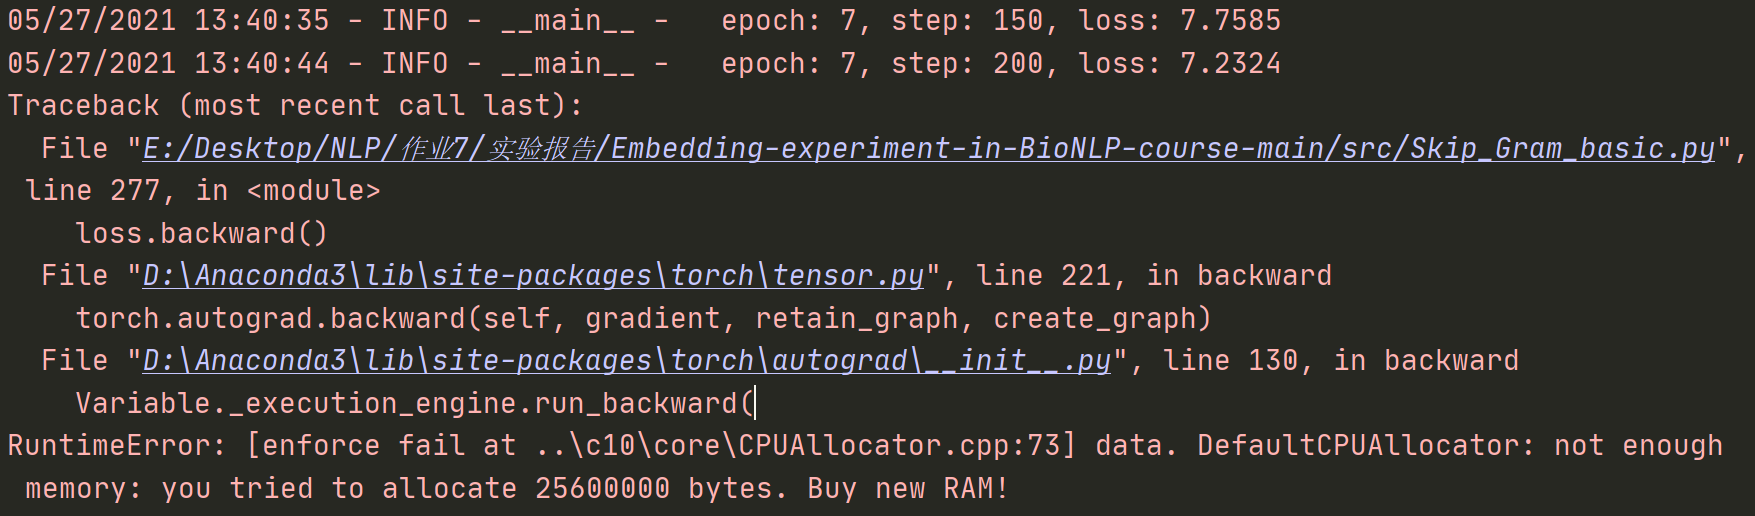
\includegraphics[scale=0.3]{./picture/error.png} %1.png是图片文件的相对路径
  \caption{} %caption是图片的标题
  \label{zzaa} %此处的label相当于一个图片的专属标志,目的是方便上下文的引用
\end{figure}
出现这个问题是因为显存不够,把其他占用显存的进程全部关闭后问题得到解决。
\section{实验结果}
\subsection{运行时间}
整个代码的运行时间从14:00:52$\rightarrow$15:21:23。足足运行了1个小时20分钟。想要降低时间可以增大学习率、减少训练次数、减小词汇规模大小等等方式。\par
Bio-BERT则快很多,从15:39:20$\rightarrow$15:46:12仅16分钟便输出结果(见图\ref{1121})。因为Bio-BERT本身是更好符合生物医药语料库的已经学好的嵌入。不需要在自己的本地进行学习。因此不论是速度还是最终呈现的效果都要比前者好很多。
\begin{figure}[H]
  \centering
  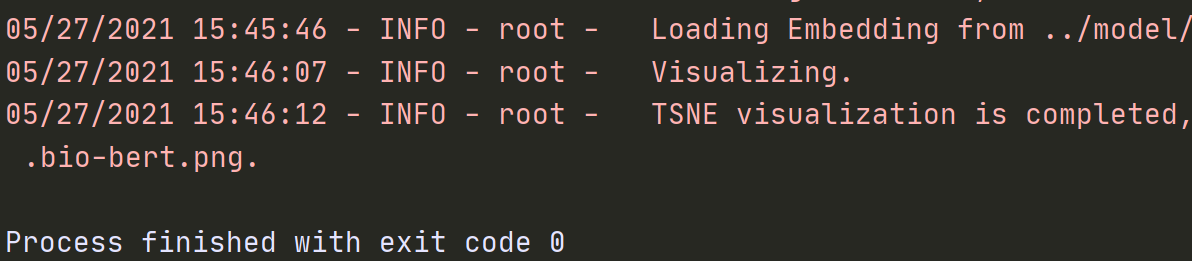
\includegraphics[scale=0.3]{./picture/result1.png} %1.png是图片文件的相对路径
  \caption{可视化完成图片已保存} %caption是图片的标题
  \label{1121} %此处的label相当于一个图片的专属标志,目的是方便上下文的引用
\end{figure}
\subsection{结果对比}
使用t-SNE进行降维可视化,变成二维空间,依旧能够保留词语之间的相似度信息(见下图\ref{sda})。
\begin{figure}[H]
  \centering
  \subfigure[Skip-gram结果]{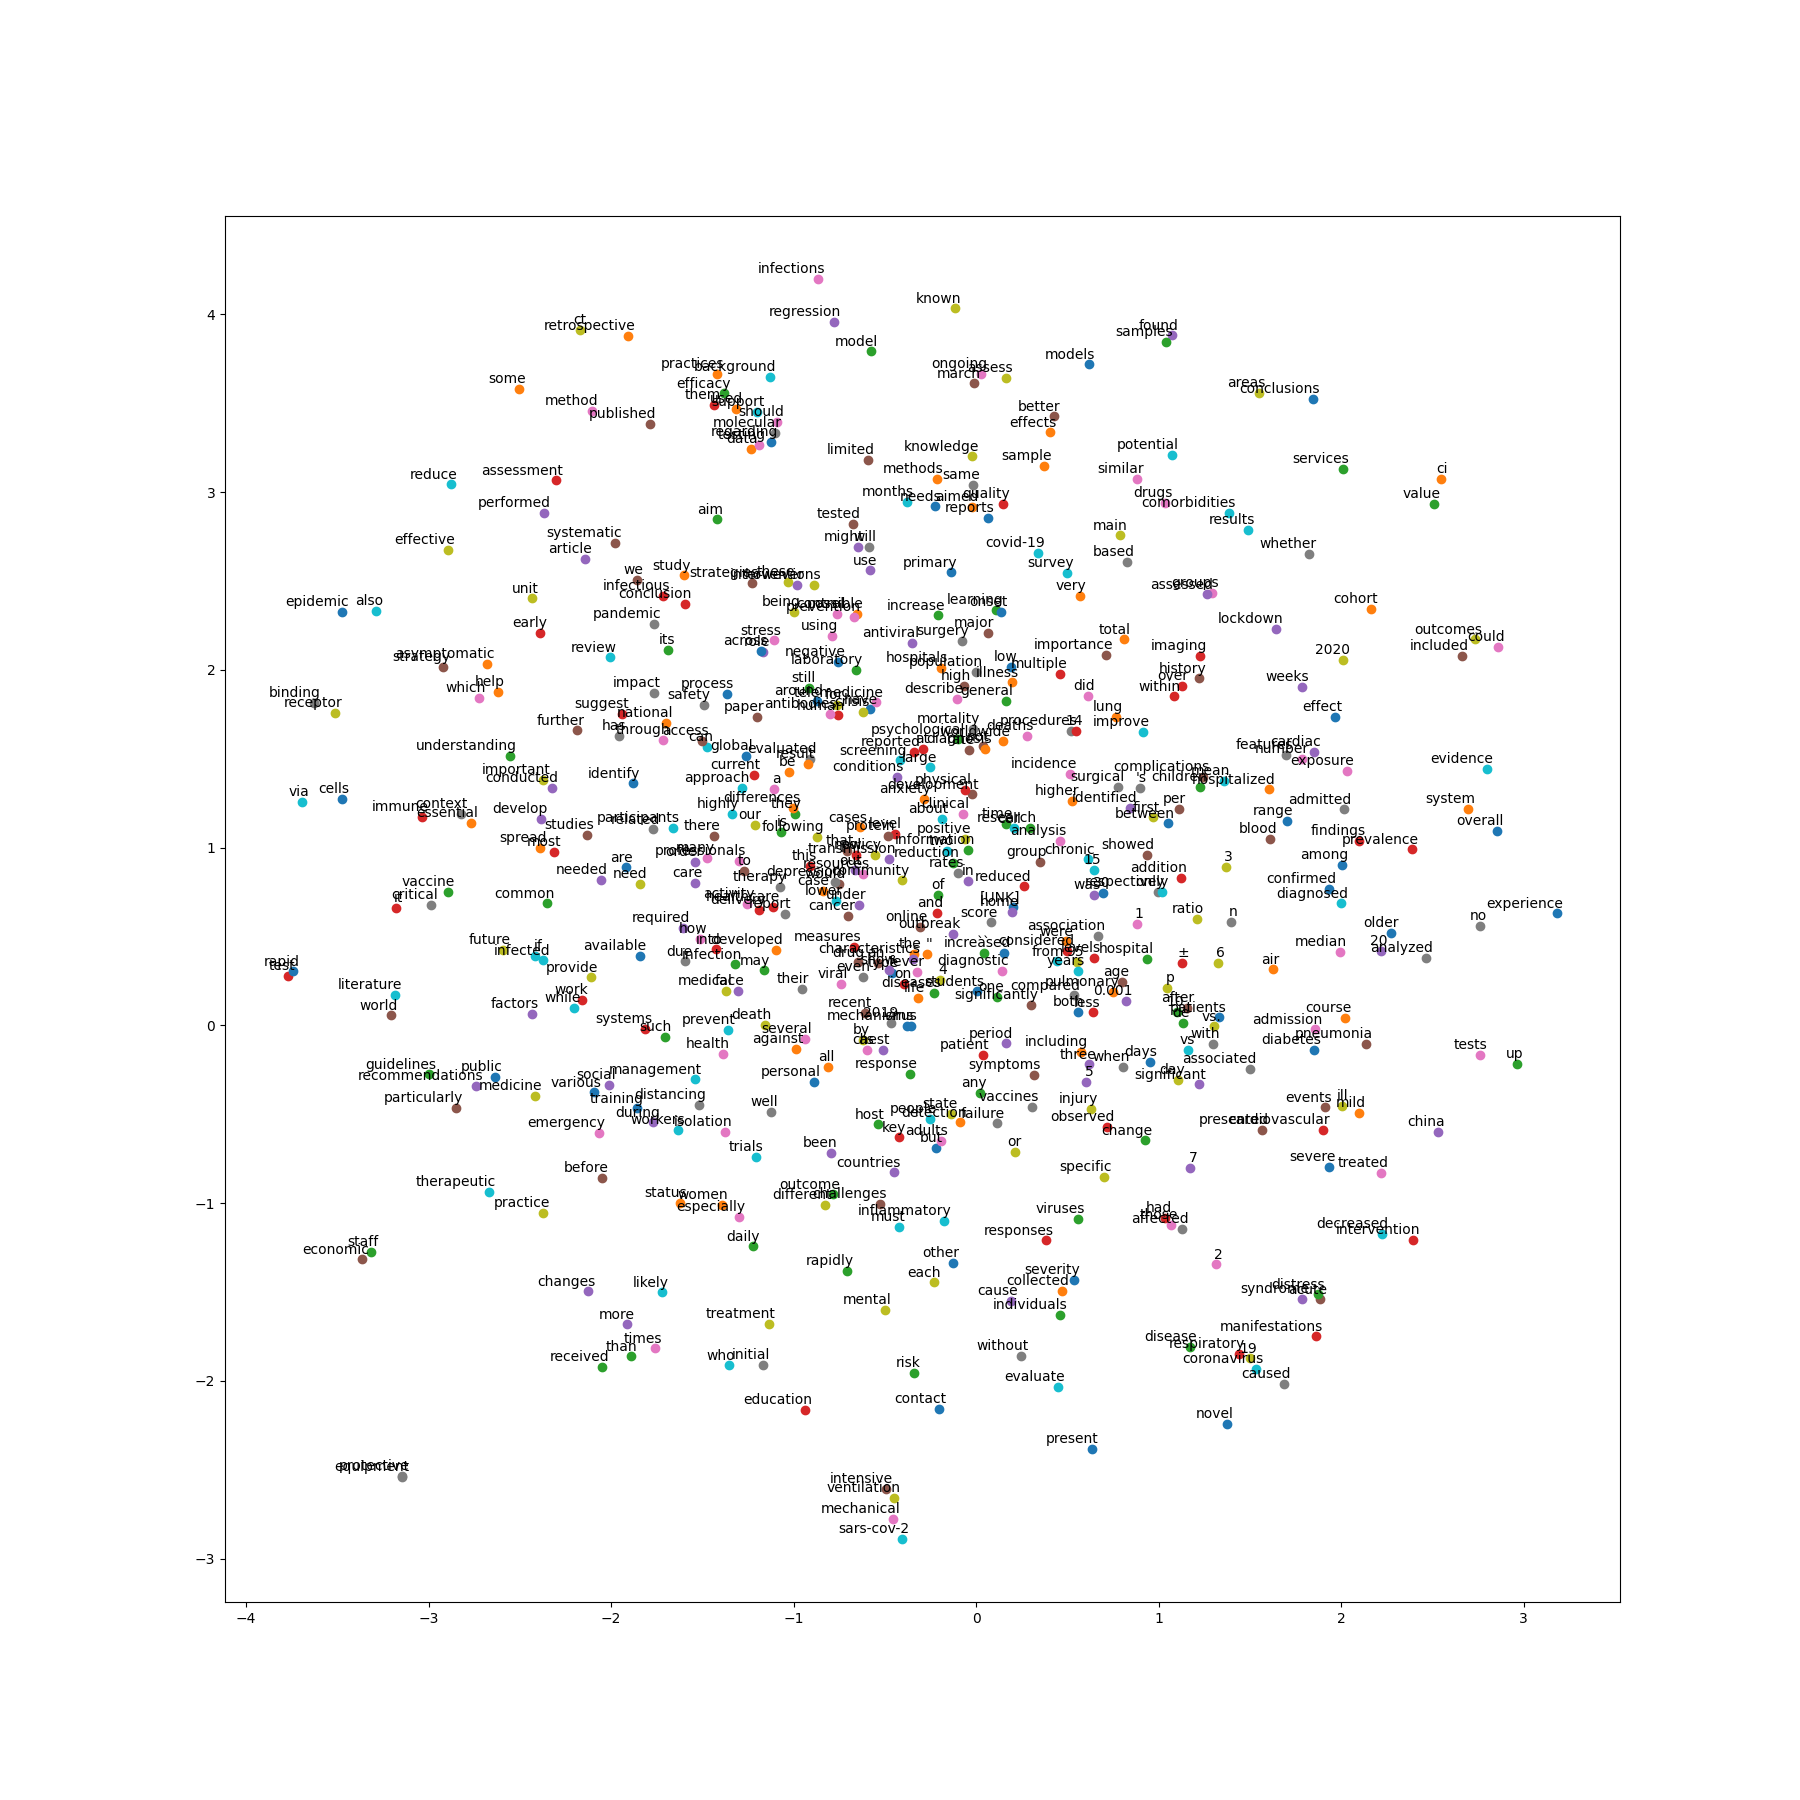
\includegraphics[width=3.1in]{picture/litcovid.tsne.png}}
  \subfigure[Bio-BERT结果]{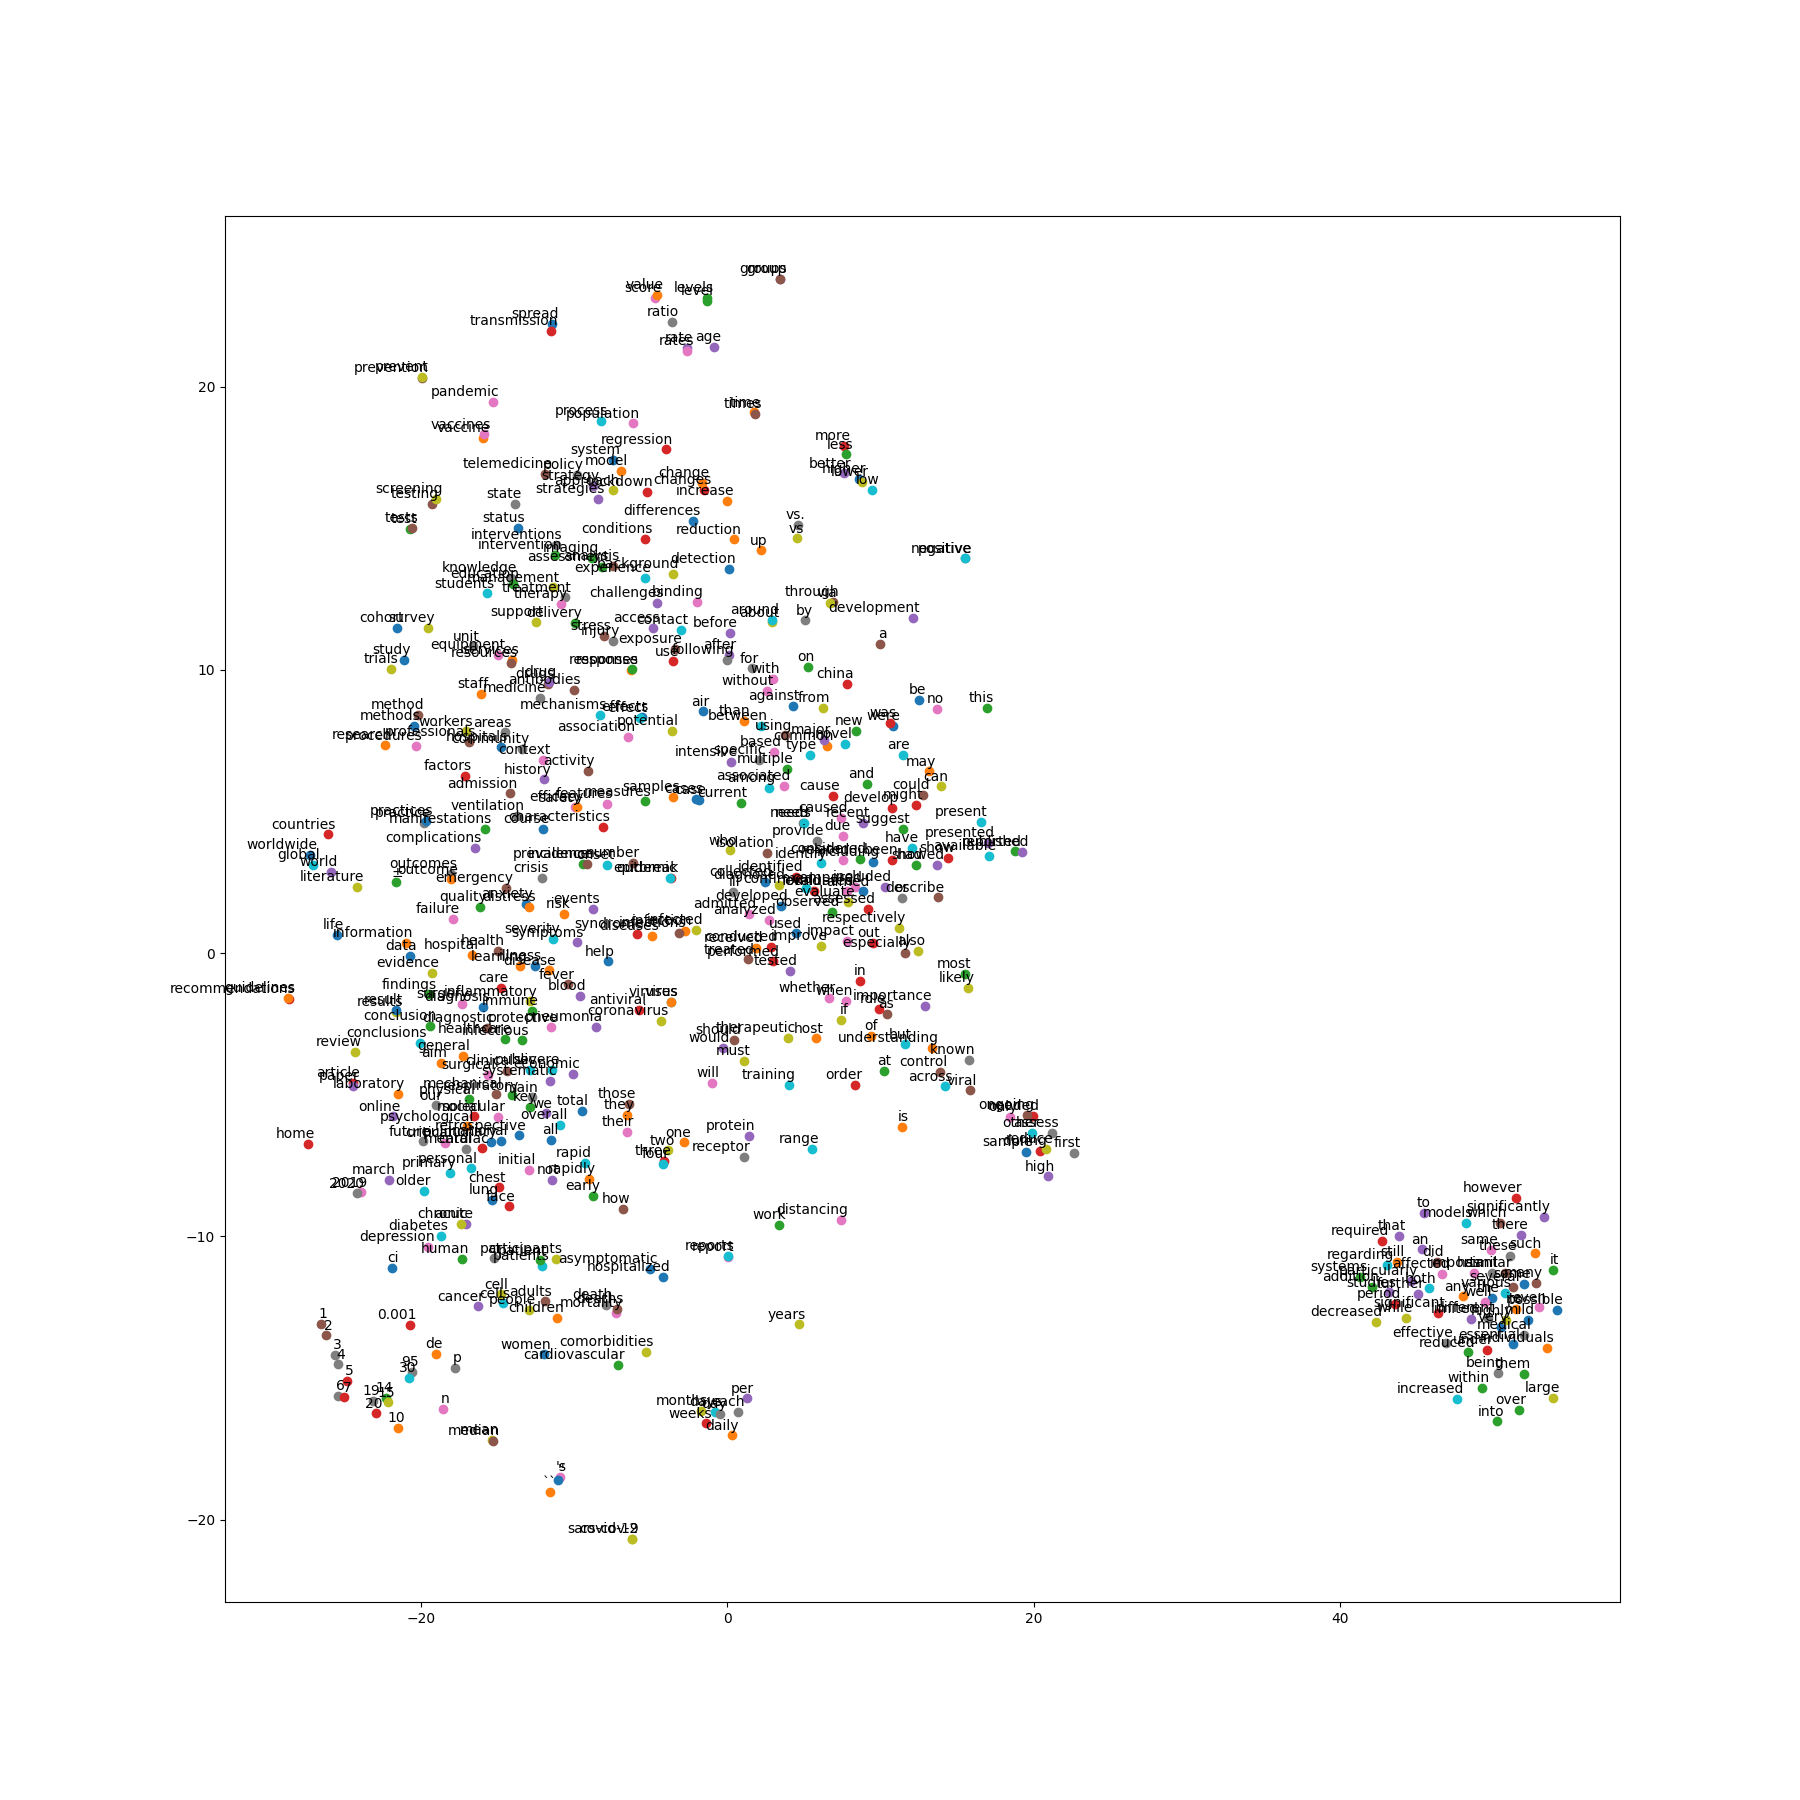
\includegraphics[width=3.1in]{picture/litcovid.tsne.bio-bert.png}}
  \caption{AGAC词干wordcloud结果}
  \label{sda}
\end{figure}
从上图对比可以看出,Bio-BERT的聚簇效果更好,通过放大图片仔细对比发现一些有趣的相似词语靠近现象。\par
\subsubsection{Skip-gram}
使用Word2Vec的Skip-gram模型自己学习到的词语嵌入见上图,明显看到呈现一个零散的球形,没有明确的聚簇的感觉。\par
不过也可以窥见一些相似的地方,比如一些数字靠的比较近,虽然没有紧紧地聚在一起,但是还是可以看出来。\par
还有就是一些副词,以ly作为词根的一些词语,比如daily,especially,rapidly,likely等也离得比较近。\par
还有就是新冠肺炎疾病相关的,比如数字19,单词novel,cronavirus,manifestations(临床表现),disease,respiratory,syndrome等等。
\subsubsection{Bio-BERT}
Bio-BERT分为两个簇,一个簇是一些名词之类,另一簇小的更多的是一些借此还有不多的代词还有动词(见下图\ref{sssa})。
而对于左边大簇而言,可以人工直观感受出其中的语义关联嵌入表示还是非常成功的。\par
表示时间的:比如2019和2020在该二维空间中几乎是完全重叠在一起的。也就是说在新冠肆虐的这两年里,年份出现的上下文非常相似。\par
表示时间的还有month,weeks,daily,per。\par
表示器官:chest胸口和lung肺的距离很近,以及face。都表示人的一些器官部位。\par
再看一些代词:those,they和their。都表示多个人。\par
情态动词:should,would,must,will也聚在一团。\par
还有数字:one,two,three,four阶梯式呈现,表明嵌入计算一定程度上能够反映其语义逻辑内容。阿拉伯数字同样如此。\par
表示数值程度的:value,rate,ratio,rates,score,levels,lavel也聚在一起。
\begin{figure}[H]
  \centering
  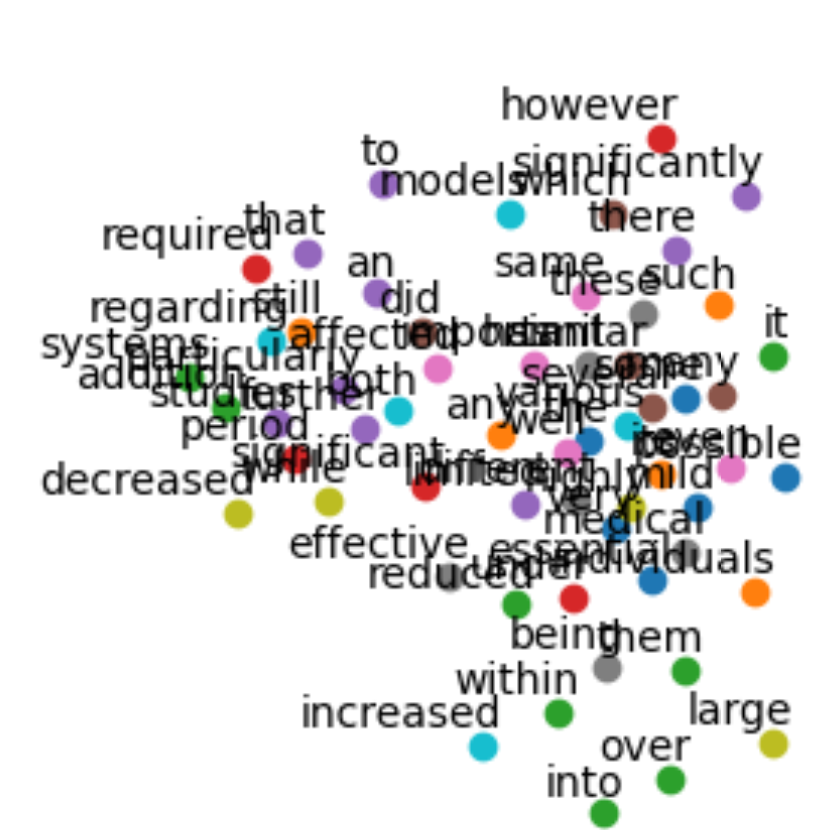
\includegraphics[scale=0.3]{./picture/另一小簇.png} %1.png是图片文件的相对路径
  \caption{另一小簇} %caption是图片的标题
  \label{sssa} %此处的label相当于一个图片的专属标志,目的是方便上下文的引用
\end{figure}
\section{github链接}
\href{https://github.com/LianzePuppet/nlp.homework7}{\underline{github链接:}}https://github.com/LianzePuppet/nlp.homework7
\section{附录}

\begin{figure}[H]
  \centering
  \subfigure[数字]{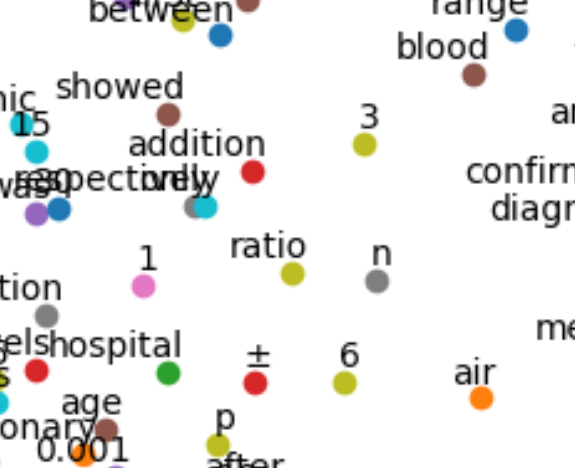
\includegraphics[width=1.5in]{picture/6.png}}
  \subfigure[以“ly”结尾副词]{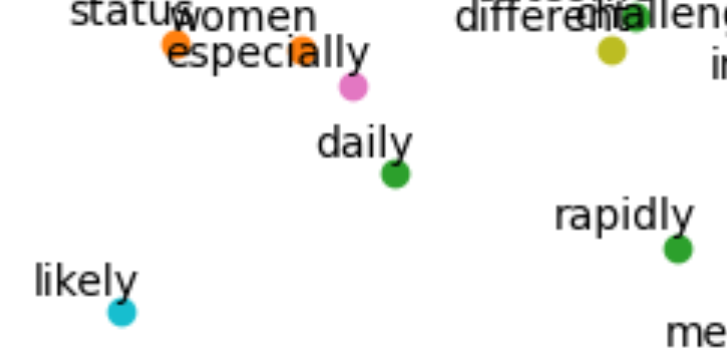
\includegraphics[width=1.5in]{picture/7.png}}
   \subfigure[新冠肺炎相关]{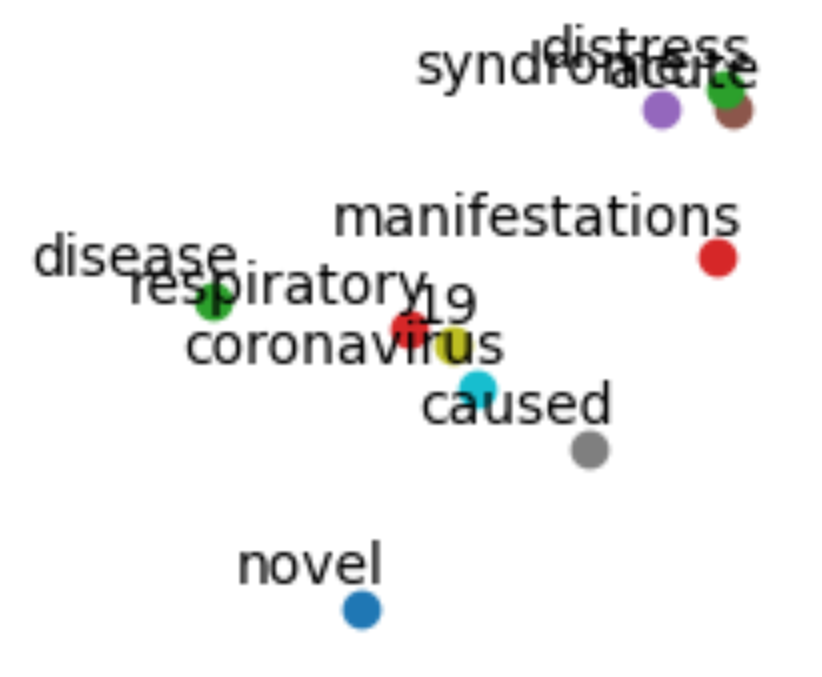
\includegraphics[width=1.5in]{picture/8.png}}
  \caption{上文提到Skip-gram得到结果的一些局部展示}
  \label{222}
\end{figure}

\begin{figure}[H]
  \centering
  \subfigure[代词]{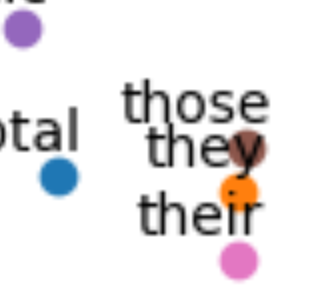
\includegraphics[width=1.5in]{picture/1.png}}
  \subfigure[年份]{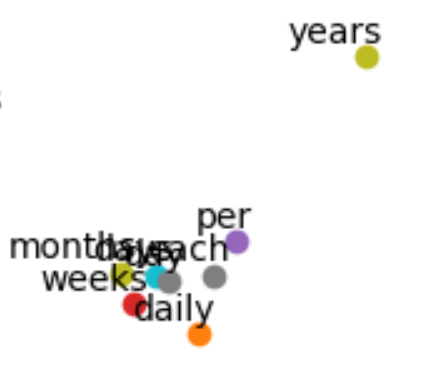
\includegraphics[width=1.5in]{picture/2.png}}
    \subfigure[数字]{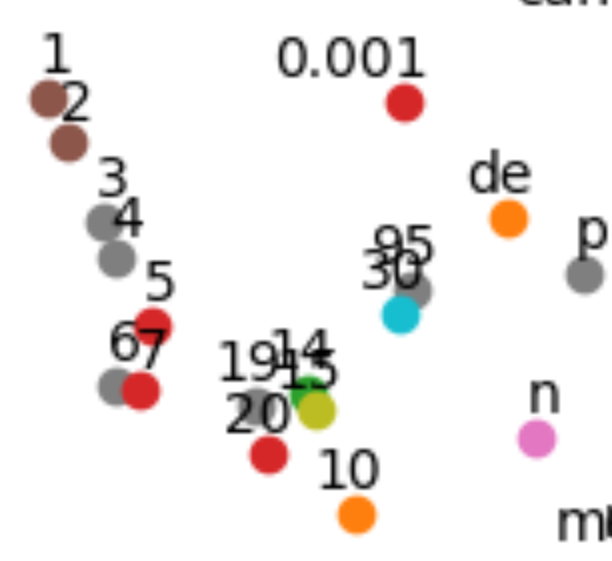
\includegraphics[width=1.5in]{picture/3.png}}
  \subfigure[数值程度]{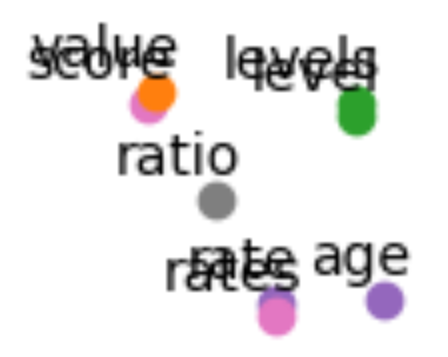
\includegraphics[width=1.5in]{picture/4.png}}
  \caption{上文提到Bio-BERT得到结果的一些局部展示}
  \label{111}
\end{figure}

\section{参考链接}
\begin{enumerate}
\item \href{https://voice.baidu.com/act/newpneumonia/newpneumonia/?from=osari_aladin_banner}{\underline{疫情实时大数据报告}}
\item \href{https://blog.csdn.net/nineship/article/details/89228497}{\underline{torch.optim}}
\item \href{https://blog.csdn.net/tsq292978891/article/details/79414512}{\underline{pytorch实现自由的数据读取-torch.utils.data的学习}}
\item \href{https://blog.csdn.net/qq_35509823/article/details/104732544}{\underline{NLP(自然语言处理):词的表示(Word representation)}}
\item \href{https://blog.csdn.net/qq_36774795/article/details/83755371}{\underline{深度学习之词向量Word Embedding总结}}
\item \href{https://www.jianshu.com/p/471d9bfbd72f}{\underline{通俗理解word2vec}}
\item \href{https://blog.csdn.net/scott198510/article/details/76099700}{\underline{t-SNE原理与推导}}
\item \href{https://blog.csdn.net/qq_35037684/article/details/108789737}{\underline{RuntimeError}}
\end{enumerate}


\end{document}
袁隆平的离世。


水稻由于其其营养价值高,加工副产品用途广作为主要的粮食作物。有关水稻文献文本挖掘方面的研究具有重要的意义。本次在Pubmed文献数据库中以rice作为关键词获取水稻文献文本。并且利用经典的词嵌入模型Word2Vec得到其中高频词的嵌入向量并进行可视化。












